% Compile from the repository root with XeLaTeX/BibTeX or the report build script.
\documentclass[11pt,a4paper]{article}
\usepackage{fontspec}
\IfFileExists{/mnt/c/Windows/Fonts/times.ttf}{
  \setmainfont{times.ttf}[Path=/mnt/c/Windows/Fonts/,BoldFont=timesbd.ttf,ItalicFont=timesi.ttf,BoldItalicFont=timesbi.ttf]
}{\IfFontExistsTF{Times New Roman}{\setmainfont{Times New Roman}}{\setmainfont{Latin Modern Roman}}}
\setsansfont{Latin Modern Sans}
\setmonofont{Latin Modern Mono}
\tracinglostchars=3
\usepackage[a4paper,margin=23mm,headheight=15pt]{geometry}
\usepackage{amsmath,amssymb,booktabs,tabularx,array,graphicx,xcolor,enumitem,fancyhdr}
\usepackage[numbers,sort&compress]{natbib}
\usepackage[unicode,hidelinks,breaklinks]{hyperref}
\usepackage{xurl}
\definecolor{navy}{HTML}{163B63}
\definecolor{slate}{HTML}{596675}
\setlength{\parindent}{0pt}
\setlength{\parskip}{0.5em}
\setlength{\emergencystretch}{3em}
\setlist{nosep,leftmargin=1.5em}
\renewcommand{\arraystretch}{1.2}
\newcolumntype{Y}{>{\raggedright\arraybackslash}X}
\newcommand{\code}[1]{{\small\nolinkurl{#1}}}
\pagestyle{fancy}\fancyhf{}
\fancyhead[L]{\small\color{slate} Memory-Bounded Teacher Scoring}
\fancyhead[R]{\small\color{slate} TECHNICAL REPORT}
\fancyfoot[C]{\thepage}

\usepackage{xeCJK}
\IfFileExists{/mnt/c/Windows/Fonts/simsun.ttc}{
  \setCJKmainfont{simsun.ttc}[Path=/mnt/c/Windows/Fonts/,BoldFont=simhei.ttf]
  \setCJKsansfont{simhei.ttf}[Path=/mnt/c/Windows/Fonts/,BoldFont=simhei.ttf]
}{\IfFontExistsTF{SimSun}{\setCJKmainfont{SimSun}[BoldFont=SimHei]\setCJKsansfont{SimHei}}{\setCJKmainfont{Noto Serif CJK SC}\setCJKsansfont{Noto Sans CJK SC}}}
\renewcommand{\refname}{参考文献}
\renewcommand{\figurename}{图}
\renewcommand{\tablename}{表}

\hypersetup{pdftitle={显存受控的教师评分},pdfauthor={Jiacheng Yu},pdfsubject={保留评分契约的 FSDP2 教师评分读出}}
\begin{document}
\hypersetup{pageanchor=false}
\begin{titlepage}
\vspace*{13mm}{\small\sffamily\bfseries\color{navy} AI INFRASTRUCTURE / 技术报告}\par
\vspace{15mm}{\LARGE\bfseries 显存受控的\\[2mm]教师评分\par}
\vspace{6mm}{\large 面向 verl FSDP2 Worker、保留评分契约的输出头读出\par}
\vspace{9mm}\hrule\vspace{7mm}
{\large\bfseries Peak allocated 降低 81.05\%}\par
\vspace{1mm}在 8,192 个投影行上，完整 Worker 调用的稠密读出为 3,596.6 MiB，分块读出为 681.6 MiB。262,144 个候选 logprob 和 8,192 行有序教师 Top-$K$ 均与稠密参考逐值一致。

\vspace{6mm}\begin{tabularx}{\linewidth}{@{}p{35mm}Y@{}}
作者 & Jiacheng Yu\\
版本 & 2026 年 10 月 31 日；简体中文\\
实验系统 & Qwen2.5-0.5B-Instruct、BF16、单 GPU、FSDP2 CPU offload\\
读出条件 & $K=32$、每块 256 行、allocator fraction 0.50\\
实验基线 & \code{ad395e94923bcf65fff4bc1eeb2e0e1505fd4f91}\\
\end{tabularx}
\vfill{\small 该百分比表示完整 Worker 调用中 PyTorch 分配器的 peak allocated，不代表整卡 VRAM 降幅。}\par
\end{titlepage}
\hypersetup{pageanchor=true}

\section*{摘要}
教师评分可能只返回紧凑分数，却仍为全部投影行和词表项生成 logits。本项目在正常 FSDP2 forward 内，将行分块前移至 Qwen2 LM Head 之前。每块计算学生候选 ID 上的全词表归一化分数和教师有序 Top-$K$，最终只保留紧凑输出。适配器可选启用，并保留固定版本 verl Worker 的共享输出头、模块 hooks 和输出布局。\cite{verl6920pinned}

在 RTX 5070 Laptop GPU 上，所述 allocator fraction 下的 $N=8192$ 实验使 PyTorch peak allocated 降低 81.05\%。另一个直接 Worker 到 Student 的实验匹配了固定反向 KL 损失、所检梯度和一次受限的最终 RMSNorm 更新。GitHub CPU 回归工作流通过 171 项测试，取消选择两项完整 Trainer runtime 对照。结果属于单 GPU 实验性执行路径优化；时延数据仅作描述，不支持通用加速结论。

\section{工程问题}
令 $N$ 为投影模型行数、$V$ 为词表大小、$K$ 为每行候选数。稠密输出头先生成 $N\times V$ logits，而响应只包含 $O(NK)$ 个值与 ID。候选集内归一化会改变评分契约：消费者需要候选 token 的全词表归一化 logprob，也需要教师自身的 Top-$K$。

行分块是已有方法；本项目的工作重点是将它接入真实 Worker，并保持评分和消费者接口。候选 logits 实现及逐行评分接口均有已有工作。\cite{indexedlogits,sglang38119}

\clearpage
\section{系统概览}
\begin{center}
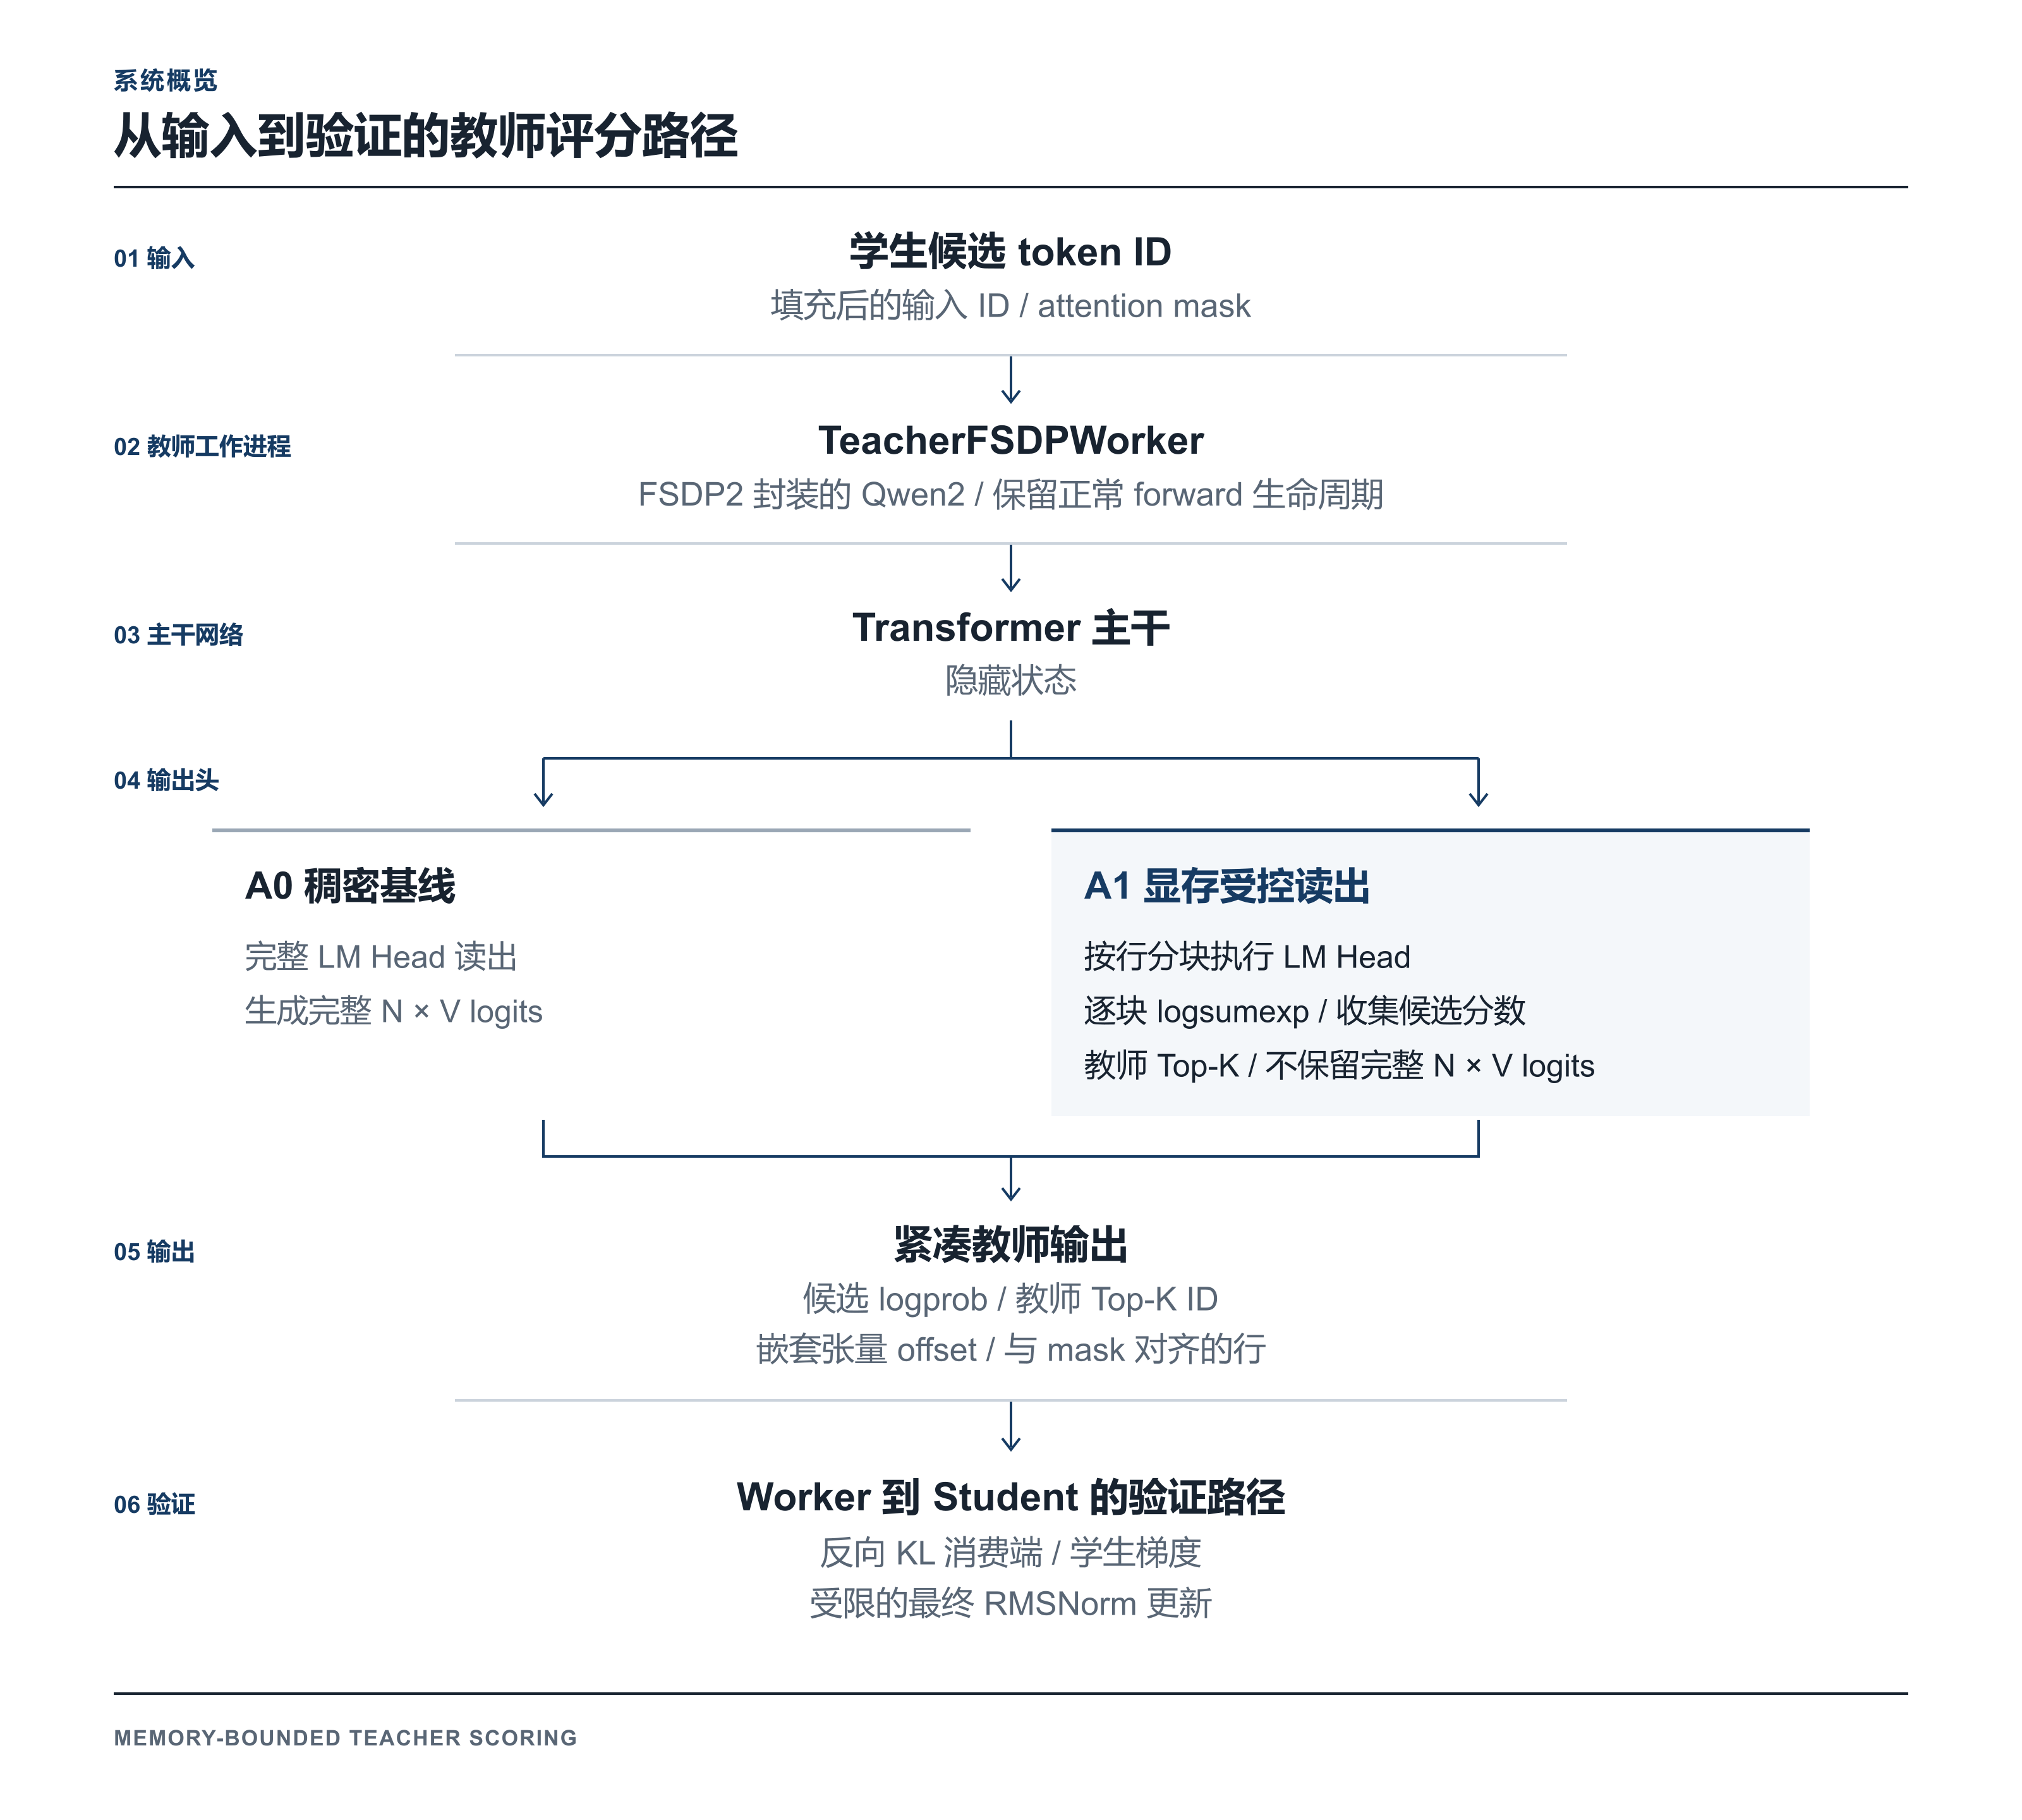
\includegraphics[width=0.98\linewidth,height=0.72\textheight,keepaspectratio]{docs/architecture/system-overview.zh-CN.png}
\end{center}
{\small\color{slate} 图 1：稠密和行分块读出共用教师执行路径与紧凑输出契约；最后一层表示独立的验证实验。}

\clearpage
\section{方法与实现}
\subsection{评分契约}
对于隐藏状态行 $h_t$、LM Head 权重 $W$、偏置 $b$ 和候选 $i$，返回分数为
\begin{equation}
z_{t,i}=h_t^{\mathsf T}W_i+b_i,\qquad
\log p_{t,i}=z_{t,i}-\log\!\sum_{j\in\mathcal V} e^{z_{t,j}}.
\end{equation}
归一化项覆盖完整词表。候选 ID 有序且允许重复，返回值保留其顺序；Worker 还返回完整词表上的教师 Top-$K$ ID，并保持嵌套张量 offset 和有效行次序。

\subsection{FSDP2 内的分块读出}
适配器在 FSDP 封装之前安装，保留参数对象以及共享的输入／输出权重。请求通过正常的外层 FSDP 模块调用进入；主干网络运行一次，随后将隐藏状态按最多 $B$ 行一块送入 LM Head 模块。每块 logits 转为 FP32，计算 log-sum-exp 和候选 gather，并保留教师 Top-$K$ ID；各块归约后丢弃，不拼接完整 $N\times V$ 结果。

同时存活的 logits 块随 $BV$ 而非 $NV$ 扩展；紧凑输出仍随 $NK$ 扩展，主干网络、模型和 FSDP 分配也仍然存在。该方法改变内存分配方式，并不消除全词表投影计算。当没有显式预算且单块覆盖全部行时，实现回退到原生稠密 forward；显式读出预算是该部分开销的估算，并非整卡硬限制。

\subsection{填充与消费者对齐}
候选 ID 使用准备好的 attention mask 散射到填充后的模型行，紧凑输出再恢复为有效行次序。适配器不对候选 ID 额外施加因果位移。消费者验证在相应预测位置使用 response mask，并将真实 Worker 输出送入固定版本的损失函数。

\clearpage
\section{实验结果}
\subsection{实验设置}
最终矩阵使用 Qwen2.5-0.5B-Instruct、BF16、单张 RTX 5070 Laptop GPU、PyTorch 2.14.1+cu130、FSDP2 CPU offload、SDPA、$K=32$、$B=256$ 和 allocator fraction 0.50。输入和候选 ID 均为合成数据。每个长度按 Dense--Chunked--Chunked--Dense 顺序运行四个独立进程；每进程预热一次、测量五次。$N$ 表示投影行数。

\begin{center}\small
\begin{tabular}{@{}rlrrrr@{}}\toprule
$N$ & 模式 & Alloc. MiB & Reserved MiB & p50 ms & p95 ms\\\midrule
1024 & Dense & 1517.1 & 2644 & 210.4 & 288.0\\
1024 & Chunked & 665.3 & 1124 & 159.4 & 187.0\\
4096 & Dense & 2409.4 & 2944 & 322.3 & 414.4\\
4096 & Chunked & 672.3 & 1130 & 318.8 & 327.5\\
8192 & Dense & 3596.6 & 3846 & 570.8 & 599.6\\
8192 & Chunked & 681.6 & 1126 & 626.3 & 944.6\\\bottomrule
\end{tabular}\par\vspace{2mm}
\end{center}
{\small\color{slate} 表 1：逐次调用的 PyTorch 分配器峰值和同步预热 Worker 耗时；每组 p50/p95 汇总十次测量。}
\begin{center}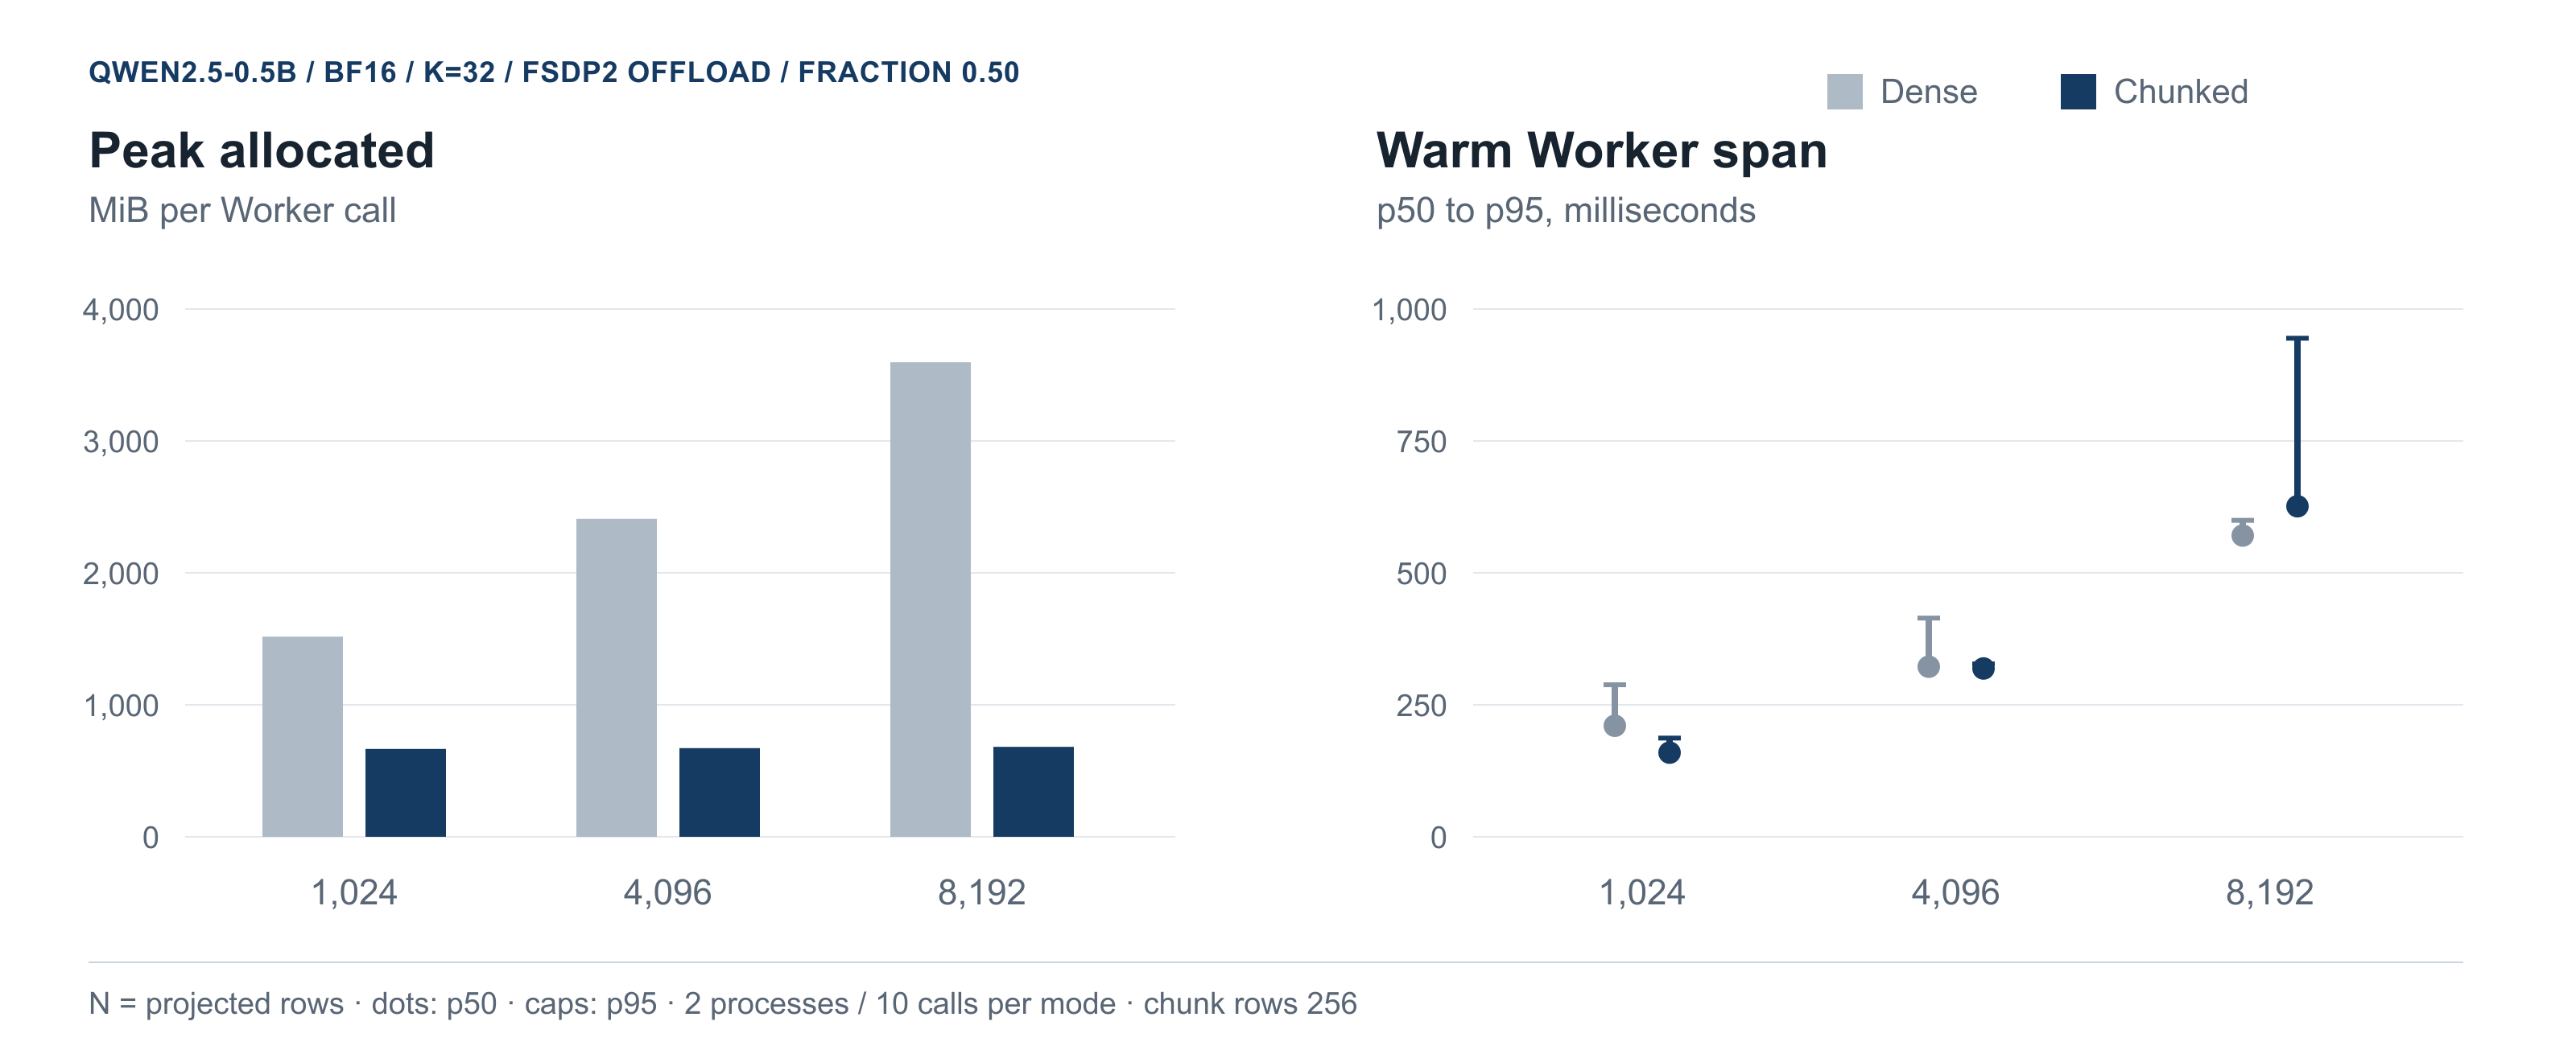
\includegraphics[width=\linewidth]{docs/figures/worker-summary.png}\end{center}
{\small\color{slate} 图 2：Peak allocated 和 p50 至 p95 的耗时范围；reserved 数值见表 1。}

\clearpage
\section{正确性与结果解释}
$N=8192$ 时，262,144 个候选 logprob 和 8,192 行有序教师 Top-$K$ 均与 Dense 参考逐值一致。最终矩阵和分块大小实验保存的 96 份紧凑输出均已重新读取，并与同长度 Dense 参考比较；对照包括输出身份、形状和 offset。

$N=8192$ 时，peak allocated 从 3,596.6 MiB 降至 681.6 MiB，降幅为 81.05\%。这是逐次调用的 PyTorch 分配器测量，并非整设备 VRAM 估计。同一 fraction 下，Dense 在 8,704 行成功、9,216 行达到分配器 OOM；Chunked 在已测最大点 32,768 行运行成功，但该点没有同长度 Dense 正确性参考。

同步计时包含诊断 hooks 和嵌套输出返回 CPU 的过程。8,192 行时 Dense 的 p50/p95 为 570.8/599.6 ms，Chunked 为 626.3/944.6 ms。进程波动和主机时钟差异限制了时延解释；这些结果不支持通用加速结论。

\subsection{Worker 到 Student 的验证}
在独立的双序列实验中，真实 Dense 和 Chunked Worker 输出进入固定版本的反向 KL 消费端，损失、学生 logits 梯度、最终 RMSNorm 梯度以及一次受限 AdamW 更新均一致。该实验使用 $K=8$、25 个有效响应预测行，只更新学生最终 RMSNorm 权重。早期实验中标量损失一致却出现梯度差异；将转换计算图与固定消费者对齐后，该测试输入中的差异消失。这是直接集成验证，不等于完整 RL 训练。

\section{当前范围与后续工作}
已测路径覆盖单 GPU FSDP2 下使用共享输出头的 Qwen2。下一阶段将扩展模型覆盖，支持 packed 变长输入，验证 FSDP1 与多 GPU／张量并行，并接入端到端 RL Trainer。早期仅计算 selected logits 的融合方案对完整评分契约仍为 NO-GO；项目历史结果保留了相应负结果。

\clearpage
\section{复现与证据}
实验代码基线为 \code{ad395e94923bcf65fff4bc1eeb2e0e1505fd4f91}；Worker 集成基于 verl \code{87cd055e872f9fdd7b976fcd797a0934b6dba265}，模型版本为 \code{7ae557604adf67be50417f59c2c2f167def9a775}。Linux／Python 3.12 的独立 Worker 锁文件固定了 105 项依赖。仓库复现指南列出环境、模型哈希、命令及实验范围。

公开结果摘要包含矩阵数据，证据清单通过 SHA-256 关联归档测量。GitHub CPU 任务在实验基线上报告 171 项通过、2 项取消选择、零跳过；它检查 CPU 回归和补丁适用性，不运行 GPU 基准。

\begin{itemize}
\item \href{https://github.com/yu830/rl-posttrain-sparse-scoring/blob/main/docs/experimental-reproduction.md}{实验复现指南}
\item \href{https://github.com/yu830/rl-posttrain-sparse-scoring/blob/main/results/worker-benchmark-summary.json}{Worker 结果摘要}与\href{https://github.com/yu830/rl-posttrain-sparse-scoring/blob/main/results/worker-evidence-manifest.json}{证据清单}
\item \href{https://github.com/yu830/rl-posttrain-sparse-scoring/actions/runs/41056928510}{GitHub Actions CPU 运行记录}
\end{itemize}

\section{结论}
将行分块边界前移至 LM Head，使该 Teacher Worker 在保留消费者所需输出的同时降低了读出期间的分配峰值。单 GPU 实测、逐值输出对照和受限 Student 更新，为下一阶段集成提供了具体依据。

\bibliographystyle{plainnat}
\bibliography{docs/reports/references}
\end{document}
